\documentclass[10pt]{beamer}
\usepackage{xcolor}

% ------------------------------------------------------------------------
% Carga de tu preámbulo personalizado (preamble.tex)
% Asegúrate de tenerlo en la misma carpeta para que \input funcione.
% ------------------------------------------------------------------------
\usetheme[progressbar=frametitle]{metropolis}
\usepackage{appendixnumberbeamer}
\usepackage{fancyvrb}
\usepackage{booktabs}
\usepackage[scale=2]{ccicons}
\usepackage{pgfplots}
\usepgfplotslibrary{dateplot}
\usepackage{type1cm}
\usepackage{lettrine}
\usepackage{ragged2e}
\usepackage{xspace}
\newcommand{\themename}{\textbf{\textsc{metropolis}}\xspace}
\usepackage{graphicx} % Allows including images
\usepackage{booktabs} % Allows the use of \toprule, \midrule and \bottomrule in tables
\usepackage[utf8]{inputenc} %solucion del problema de los acentos.
\usepackage{xcolor}
\definecolor{LightGray}{gray}{0.9}

\usepackage{minted}
\usemintedstyle{tango}
\newcommand{\mypyfile}[1]{\inputminted[linenos=true, fontsize=\footnotesize, frame=lines, framesep=5\fboxrule,framerule=1pt]{python}{#1}}

\setminted[python]{breaklines,frame=lines,framesep=2mm,baselinestretch=1.2,bgcolor=LightGray,linenos, fontsize=\footnotesize} % obeytabs=true, tabsize=2, showtabs=true}

%%%%%%%%%%%%%%%%%%%%%%%%%%%%%%%%%%%%%%%%%%%%%%%%%%%%%%%%%%%%%%%%%%%%%%%%%%%%%%%%%%%%%%
\setbeamercolor{progress bar}{fg=blue!50!black,bg=white!50!black}
\setbeamercolor{title separator}{fg=red!50!black,bg=white!50!black}
\setbeamercolor{frametitle}{fg=white!80!black,bg=red!50!black}
\title[PCFI161]{Programaci\'on para F\'isica y Astronom\'ia}
\subtitle{Departamento de Física.}

\newcommand{\myfront}{
\author[PCFI161]{Corodinadora: C Loyola \\ Profesoras/es C Loyola / C Femenías / Y Navarrete / C Ruiz}
\institute[UNAB]{Universidad Andrés Bello}
\date{Primer Semestre 2025}
}

\titlegraphic{%
  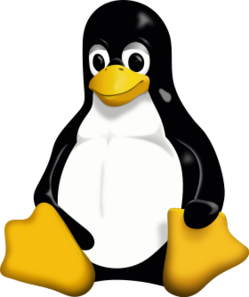
\includegraphics[width=.08\textwidth]{logo-tux.png}\hfill
  
\includegraphics[width=.3\textwidth]{logo-unab.png}\hfill
  
\includegraphics[width=.08\textwidth]{logo-python.png}
}

\makeatletter
\setbeamertemplate{title page}{
  \begin{minipage}[b][\paperheight]{\textwidth}
    \vfill%
    \ifx\inserttitle\@empty\else\usebeamertemplate*{title}\fi
    \ifx\insertsubtitle\@empty\else\usebeamertemplate*{subtitle}\fi
    \usebeamertemplate*{title separator}
    \ifx\beamer@shortauthor\@empty\else\usebeamertemplate*{author}\fi
    \ifx\insertdate\@empty\else\usebeamertemplate*{date}\fi
    \ifx\insertinstitute\@empty\else\usebeamertemplate*{institute}\fi
    \vfill
    \ifx\inserttitlegraphic\@empty\else\inserttitlegraphic\fi
    \vspace*{1cm}
  \end{minipage}
}
\makeatother


\makeatletter
\setlength{\metropolis@titleseparator@linewidth}{2pt}
\setlength{\metropolis@progressonsectionpage@linewidth}{2pt}
\setlength{\metropolis@progressinheadfoot@linewidth}{2pt}
\makeatother


\begin{document}

% ------------------------------------------------------------------------
% Portada personalizada (ejemplo \myfront si está definido en tu preámbulo)
% ------------------------------------------------------------------------
\myfront{}

% ------------------------------------------------------------------------
% Slide 1: Título de la Sesión
% ------------------------------------------------------------------------
\begin{frame}
  \titlepage
  % Por ejemplo:
  % \title{Semana 4 - Sesión 2 (Sesión 8): Taller de Funciones, Módulos y Librerías Externas}
\end{frame}

% ------------------------------------------------------------------------
% Slide 2: Índice / Tabla de Contenidos
% ------------------------------------------------------------------------
\begin{frame}
  \frametitle{Resumen - Semana 3, Sesión 2 (Sesión 6)}
  \tableofcontents
\end{frame}

% ------------------------------------------------------------------------
% Configuración de bloques
% ------------------------------------------------------------------------
\metroset{block=fill}

% ----------------------------------------------------------------------------------------
% SECCIÓN 1: Introducción y Repaso
% ----------------------------------------------------------------------------------------
\section{Introducción y Repaso}

% ------------------------------------------------------------------------
% Slide 3: Recapitulación de la Sesión 6
% ------------------------------------------------------------------------
\begin{frame}{Recapitulación de la Sesión Anterior (Sesión 6)}
  \begin{itemize}
    \item \textbf{Semana 3, Sesión 2 (Sesión 6)} se centró en:
      \begin{itemize}
        \item \textbf{Funciones}: sintaxis (\texttt{def}), parámetros, valores por defecto, alcance de variables.
        \item \textbf{Módulos y Paquetes}: cómo organizar el código en archivos \texttt{.py} y carpetas.
        \item Ejemplos de proyectos pequeños con \texttt{import} y definición de funciones útiles.
      \end{itemize}
    \item \textbf{Objetivo de hoy}: Ampliar la práctica con funciones y módulos, e \textbf{introducir el uso de librerías externas} (vía \texttt{pip} o Colab).
  \end{itemize}
\end{frame}

% ------------------------------------------------------------------------
% Slide 4: Objetivos de la Sesión 5
% ------------------------------------------------------------------------
\begin{frame}{Objetivos de la Sesión 5}
  \begin{itemize}
    \item \textbf{Profundizar} en el flujo de trabajo al crear y reutilizar módulos en Python.
    \item \textbf{Explorar} la instalación de librerías externas (\texttt{pip}, Google Colab).
    \item \textbf{Diseñar} una actividad grupal donde se combine la creación de funciones propias con el uso de librerías de terceros.
    \item \textbf{Fomentar} la colaboración y la discusión sobre buenas prácticas de organización.
  \end{itemize}
\end{frame}

% ----------------------------------------------------------------------------------------
% SECCIÓN 2: Repaso Rápido de Módulos y Paquetes
% ----------------------------------------------------------------------------------------
\section{Módulos y Paquetes}

% ------------------------------------------------------------------------
% Slide 5: Estructura de un Proyecto Simple
% ------------------------------------------------------------------------
\begin{frame}{Estructura Básica de un Proyecto}
  \begin{itemize}
    \item \textbf{Carpetas y librerías}: Organiza tu proyecto en carpetas y utiliza librerías conocidas para funcionalidades específicas.
    \item \texttt{main.py}: Archivo principal que orquesta la lógica del programa.
    \item Ejemplo de estructura:
      \begin{itemize}
        \item \texttt{main.py}: Código principal.
        \item \texttt{data/}: Carpeta para almacenar datos.
        \item \texttt{requirements.txt}: Lista de librerías necesarias.
      \end{itemize}
    \item \textbf{Ventaja}: Facilita la mantenibilidad, escalabilidad y reutilización del código.
  \end{itemize}
\end{frame}



% ------------------------------------------------------------------------
% Slide 6: Importar Librerías Conocidas
% ------------------------------------------------------------------------
\begin{frame}[fragile]{Formas de Importar Librerías Conocidas}
\textbf{Import completo}: Útil para acceder a todas las funcionalidades de una librería.
\begin{minted}[fontsize=\tiny]{python}
import numpy as np
arr = np.array([1, 2, 3])
print(np.mean(arr))
\end{minted}

\textbf{From / Import}: Importa solo las funciones necesarias.
\begin{minted}[fontsize=\tiny]{python}
from math import sqrt
resultado = sqrt(16)
print(resultado)
\end{minted}

\textbf{Import renombrado}: Simplifica el uso de librerías con nombres largos.
\begin{minted}[fontsize=\tiny]{python}
import pandas as pd
df = pd.DataFrame({"A": [1, 2], "B": [3, 4]})
print(df)
\end{minted}

\end{frame}

% ----------------------------------------------------------------------------------------
% SECCIÓN 3: Librerías Externas y pip
% ----------------------------------------------------------------------------------------
\section{Librerías Externas}

% ------------------------------------------------------------------------
% Slide 7: ¿Por qué usar Librerías Externas?
% ------------------------------------------------------------------------
\begin{frame}{¿Por qué Librerías Externas?}
  \begin{itemize}
    \item \textbf{Ahorra tiempo}: aprovechas código ya probado por la comunidad.
    \item \textbf{Funcionalidades avanzadas}: Desde manejo de redes hasta machine learning.
    \item \textbf{Ejemplos}: \texttt{requests} para peticiones web, \texttt{numpy} para cálculo numérico, \texttt{pandas} para data frames, etc.
    \item \textbf{Comunidad activa}: librerías mantenidas, actualizaciones frecuentes.
  \end{itemize}
\end{frame}

% ------------------------------------------------------------------------
% Slide 8: Instalación con pip
% ------------------------------------------------------------------------
\begin{frame}[fragile]{Instalación con \texttt{pip}}
  \begin{itemize}
    \item \textbf{pip}: el gestor de paquetes oficial de Python.
    \item Comando general en terminal:
    \begin{minted}{bash}
      pip install nombre_paquete
    \end{minted}
    \item Si usas \textbf{Google Colab}, puedes instalar temporalmente en una celda:
    \begin{minted}{python}
!pip install nombre_paquete
    \end{minted}
    \item La librería quedará disponible para importarse en el resto del entorno (hasta reiniciar).
  \end{itemize}
\end{frame}

% ------------------------------------------------------------------------
% Slide 9: Ejemplo: Instalando \texttt{requests} en Colab
% ------------------------------------------------------------------------
\begin{frame}[fragile]{Ejemplo: \texttt{requests} en Colab}
\begin{minted}{python}
# En una celda de Colab:
!pip install requests

import requests

resp = requests.get("https://api.github.com")
print(resp.status_code)
print(resp.json())
\end{minted}
\begin{itemize}
  \item \textbf{Uso real}: Conectarse a APIs, descargar datos, etc.
  \item \textbf{Sugerencia}: Manejar casos de error (\texttt{resp.status\_code != 200}).
\end{itemize}
\end{frame}

% ------------------------------------------------------------------------
% Slide 10: Ejemplo: Instalando \texttt{numpy}
% ------------------------------------------------------------------------
\begin{frame}[fragile]{Ejemplo: \texttt{numpy} Básico}
  \begin{itemize}
    \item Instalación desde terminal local:
    \begin{minted}{bash}
      pip install numpy
    \end{minted}
    \item Uso en el código:
    \begin{minted}{python}
import numpy as np
arr = np.array([1, 2, 3, 4])
print(arr * 2)  # [2 4 6 8]
    \end{minted}
    \item \textbf{NumPy} es la base de muchas librerías científicas en Python.
    \item \textbf{Operaciones vectorizadas}: eficiencia y simplicidad.
  \end{itemize}
\end{frame}


% ----------------------------------------------------------------------------------------
% SECCIÓN 4: Ejercicios práctivos Integrados
% ----------------------------------------------------------------------------------------
\section{Ejercicios Prácticos Integrados}


% ------------------------------------------------------------------------
% Slide 10: Ejercicio 1 - Análisis de Temperaturas
% ------------------------------------------------------------------------
\begin{frame}{Ejercicio 1: \hfill \textcolor{red}{$\clubsuit$} \\ Análisis de Temperaturas}
  \begin{block}{Enunciado}
    \begin{itemize}
      \item Crear una función \texttt{clasificar\_temperatura(temp)} que clasifique una temperatura en grados Celsius:
        \begin{itemize}
          \item $< 0\,^\circ\mathrm{C}$: "Estado sólido (hielo)"
          \item $0\,^\circ\mathrm{C}$ -- $100\,^\circ\mathrm{C}$: "Estado líquido (agua)"
          \item $> 100\,^\circ\mathrm{C}$: "Estado gaseoso (vapor)"
        \end{itemize}
      \item Crear un programa principal (.ipynb de la clase) que:
        \begin{itemize}
          \item Pida al usuario 3 temperaturas diferentes
          \item Use la función para clasificar cada temperatura
          \item Muestre el resultado para cada temperatura ingresada
        \end{itemize}
    \end{itemize}
  \end{block}
  \textbf{Conceptos:} Funciones básicas, condicionales if-elif-else.\\
  \textbf{Física relevante:} Estados de la materia, puntos de cambio de fase.
\end{frame}

% ------------------------------------------------------------------------
% Slide 11: Ejercicio 2 - Conversor de Unidades Simple
% ------------------------------------------------------------------------
\begin{frame}{Ejercicio 2: \hfill \textcolor{red}{$\clubsuit$} \\ Conversor de Unidades Simple}
  \begin{block}{Enunciado}
    \begin{itemize}
      \item Crear un archivo \texttt{convertidor.py} con dos funciones:
        \begin{itemize}
          \item \texttt{celsius\_a\_fahrenheit(c)} → retorna $F = C \times 9/5 + 32$
          \item \texttt{metros\_a\_pies(m)} → retorna $pies = metros \times 3.281$
        \end{itemize}
      \item En otro archivo (.ipynb de la clase):
        \begin{itemize}
          \item Importar las funciones del módulo \texttt{convertidor}
          \item Pedir al usuario un valor y la conversión deseada (1: C→F, 2: m→pies)
          \item Mostrar el resultado de la conversión
        \end{itemize}
    \end{itemize}
  \end{block}
  
  \textbf{Conceptos:} Módulos básicos, importación, funciones simples, condicionales.\\
  \textbf{Física relevante:} Sistemas de unidades y conversiones básicas.
\end{frame}

% ------------------------------------------------------------------------
% Slide 12: Ejercicio 3 - Calculadora de Caída Libre
% ------------------------------------------------------------------------
\begin{frame}{Ejercicio 3: \hfill \textcolor{red}{$\clubsuit$} \\ Calculadora de Caída Libre}
  \begin{block}{Enunciado}
    \begin{itemize}
      \item Crear una función \texttt{posicion\_caida(t, h0, g=9.8)}:
        \begin{itemize}
          \item Calcula posición usando $h = h0 - \frac{1}{2}g \cdot t^2$
          \item Parámetros: t (tiempo), h0 (altura inicial), g (gravedad)
        \end{itemize}
      \item Crear un programa principal (.ipynb de la clase) que:
        \begin{itemize}
          \item Pida al usuario la altura inicial de un objeto
          \item Calcular y mostrar la posición cada segundo (de 0 a 5 segundos)
          \item Imprimir "¡El objeto tocó el suelo!" si la posición es menor o igual a 0
        \end{itemize}
    \end{itemize}
  \end{block}
  
  \textbf{Conceptos:} Funciones con parámetros por defecto, bucle for simple, condicionales básicos.\\
  \textbf{Física relevante:} Cinemática básica, caída libre.
\end{frame}

% ------------------------------------------------------------------------
% Slide 13: Ejercicio 4 - Estadísticas Básicas
% ------------------------------------------------------------------------
\begin{frame}{Ejercicio 4: \hfill \textcolor{red}{$\clubsuit$} \\ Estadísticas Básicas}
  \begin{block}{Enunciado}
    \begin{itemize}
      \item Crear un módulo \texttt{estadistica.py} con una función:
        \begin{itemize}
          \item \texttt{calcular\_promedio(valores)} - retorna la media aritmética
        \end{itemize}
      \item Crear un programa principal (.ipynb de la clase) que:
        \begin{itemize}
          \item Importe la función desde el módulo
          \item Pida al usuario que ingrese 5 mediciones de temperatura
          \item Valide que las entradas sean números (use un bucle while si es necesario)
          \item Calcule y muestre el promedio de las mediciones
        \end{itemize}
    \end{itemize}
  \end{block}
  
  \textbf{Conceptos:} Módulos básicos, funciones simples, listas, bucle for, validación básica.\\
  \textbf{Física relevante:} Mediciones de temperatura, promedio de datos experimentales.
\end{frame}

% ------------------------------------------------------------------------
% Slide 14: Ejercicio 5 - Mini-Calculadora Científica
% ------------------------------------------------------------------------
\begin{frame}{Ejercicio 5: \hfill \textcolor{red}{$\clubsuit$} \\ Mini-Calculadora Científica}
  \begin{block}{Enunciado}
    \begin{itemize}
      \item Crear un módulo \texttt{calculadora.py} con dos funciones:
        \begin{itemize}
          \item \texttt{energia\_cinetica(masa, velocidad)} - calcula $E_c = \frac{1}{2}mv^2$
          \item \texttt{energia\_potencial(masa, altura, g=9.8)} - calcula $E_p = mgh$
        \end{itemize}
      \item Crear un programa principal (.ipynb de la clase) que:
        \begin{itemize}
          \item Importar las funciones del módulo
          \item Presentar un menú simple con opciones (1: E. Cinética, 2: E. Potencial)
          \item Pedir los datos necesarios según la opción elegida
          \item Mostrar el resultado del cálculo
        \end{itemize}
    \end{itemize}
  \end{block}
  
  \textbf{Conceptos:} Módulos básicos, funciones, menú simple con if-elif, entrada de usuario.\\
  \textbf{Física relevante:} Energía cinética y potencial, conservación de energía mecánica.
\end{frame}


% ----------------------------------------------------------------------------------------
% SECCIÓN 4: Actividad Práctica
% ----------------------------------------------------------------------------------------
\section{Tarea 2}

% ------------------------------------------------------------------------
% Slide 15: Tarea Pregunta 1 - Calculadora de Movimiento Simple
% ------------------------------------------------------------------------
\begin{frame}{Tarea Pregunta 1: \hfill \textcolor{blue}{$\bigstar$} \\ Calculadora de Movimiento Simple}
  \begin{block}{Enunciado}
    \begin{itemize}
      \item Definir una función \texttt{calcular\_posiciones(velocidad\_inicial, tiempo\_max, intervalo=1)} que:
        \begin{itemize}
          \item Calcule las posiciones de un objeto en movimiento rectilíneo uniforme
          \item La posición se determina por $x(t) = v \cdot t$ (donde $v$ es la velocidad constante)
          \item Use un bucle \texttt{for} para calcular la posición en cada intervalo de tiempo desde 0 hasta \texttt{tiempo\_max}
          \item Si la posición supera 100 unidades, incluya un mensaje "Fuera de rango" junto al valor
        \end{itemize}
      \item Ejemplo de uso:
        \begin{itemize}
          \item \texttt{calcular\_posiciones(10, 5)} debería calcular la posición cada segundo durante 5 segundos
          \item \texttt{calcular\_posiciones(15, 10, 0.5)} debería calcular la posición cada medio segundo durante 10 segundos
        \end{itemize}
    \end{itemize}
  \end{block}
  
  \textbf{Entrega:} Notebook (\texttt{.ipynb}) con el código y ejemplos de uso de la función.\\
  \textbf{Física relevante:} Cinemática básica, movimiento rectilíneo uniforme.
\end{frame}

% ------------------------------------------------------------------------
% Slide 16: Tarea Pregunta 2 - Filtrado y Análisis de Datos Experimentales
% ------------------------------------------------------------------------
\begin{frame}{Tarea Pregunta 2: \hfill \textcolor{blue}{$\bigstar$} \\ Filtrado y Análisis de Datos Experimentales}
  \begin{block}{Enunciado}
    \begin{itemize}
      \item Definir una función \texttt{procesar\_datos(datos, umbral\_min=None, umbral\_max=None)} que:
        \begin{itemize}
          \item Filtre valores atípicos fuera del rango [\texttt{umbral\_min}, \texttt{umbral\_max}]
          \item Si \texttt{umbral\_min} es \texttt{None}, calcule automáticamente como $media - 2*desviacion$
          \item Si \texttt{umbral\_max} es \texttt{None}, calcule automáticamente como $media + 2*desviacion$
          \item Use \texttt{if} para verificar los umbrales
          \item Use \texttt{for} y \texttt{continue} para saltar valores fuera de rango
          \item Retorne la lista de valores filtrados
        \end{itemize}
    \end{itemize}
  \end{block}
  
  \textbf{Entrega:} Notebook (\texttt{.ipynb}) con implementación y pruebas de las funciones.\\
  \textbf{Física relevante:} Tratamiento de datos experimentales, análisis estadístico en mediciones.
\end{frame}



% ----------------------------------------------------------------------------------------
% SECCIÓN 5: Conclusiones
% ----------------------------------------------------------------------------------------
\section{Conclusiones y Próximos Pasos}

% ------------------------------------------------------------------------
% Slide 21: Análisis General
% ------------------------------------------------------------------------
\begin{frame}{Análisis General de la Actividad}
  \begin{itemize}
    \item Ventajas de \textbf{combinar módulos propios con librerías externas}:
      \begin{itemize}
        \item Reutilización de código (módulos).
        \item Potencia y robustez (librerías de terceros).
      \end{itemize}
    \item Importancia de la \textbf{organización de archivos} y de un \textbf{flujo de trabajo} claro.
    \item Manejar \textbf{entornos virtuales} (en local) es otra buena práctica (tema futuro).
  \end{itemize}
\end{frame}

% ------------------------------------------------------------------------
% Slide 22: Recomendaciones de Estudio
% ------------------------------------------------------------------------
\begin{frame}{Recomendaciones de Estudio}
  \begin{itemize}
    \item Revisar la \textbf{documentación oficial} de \texttt{pip} y \texttt{virtualenv}.
    \item Explorar \textbf{PyPI} (\url{https://pypi.org/}) para descubrir librerías útiles.
    \item Practicar la creación de \textbf{módulos} en proyectos pequeños.
    \item Investigar qué librerías podrían ser útiles para futuros trabajos de Física/Astronomía (p.e. \texttt{astropy}, \texttt{scipy}).
  \end{itemize}
\end{frame}

% ------------------------------------------------------------------------
% Slide 23: Visión de la Próxima Sesión
% ------------------------------------------------------------------------
\begin{frame}{Próxima Sesión}
  \begin{itemize}
    \item \textbf{Sesion 7 (Semana 4)}: Aplicaciones profundas de Unidades I y II.
    \item \textbf{Recomendación}:
      \begin{itemize}
        \item Revisa todos los conceptos vistos: Sintaxis, Estructuras de Control, Funciones, Módulos.
        \item Práctica con ejercicios y ejemplos de exámenes pasados (si los hubiera).
      \end{itemize}
  \end{itemize}
  \vspace{0.3cm}
  \textbf{¡Prepárate para la evaluación!}
\end{frame}

% ------------------------------------------------------------------------
% Slide 24: Recursos Adicionales
% ------------------------------------------------------------------------
\begin{frame}{Recursos Adicionales}
  \begin{itemize}
    \item \href{https://packaging.python.org/tutorials/installing-packages/}{\textbf{Official Python Packaging Tutorial}}
    \item \href{https://docs.python.org/3/library/}{\textbf{Documentación de la Biblioteca Estándar de Python}}
    \item \href{https://pypi.org/}{\textbf{PyPI}} - Python Package Index
    \item \href{https://numpy.org/doc/}{\textbf{Numpy Docs}}
    \item \href{https://matplotlib.org/stable/}{\textbf{Matplotlib Docs}}
  \end{itemize}
\end{frame}

% ------------------------------------------------------------------------
% Slide 25: Cierre de la Sesión
% ------------------------------------------------------------------------
\begin{frame}{Cierre de la Sesión}
  \huge{\centerline{¡Muchas gracias y éxito en su práctica!}}
  \vspace{0.4cm}
  \normalsize
  \begin{itemize}
    \item Recuerden subir su trabajo a Google Drive o repositorio compartido.
    \item ¡Sigan explorando librerías externas y creando módulos propios!
  \end{itemize}
\end{frame}

\end{document}

